\noindent{\begin{center}
\fbox{
\begin{minipage}{0.95\textwidth}
    \vspace{2pt}
    \begin{center}
    \textbf{\textit{CELEBRAZIONI per la Madonna delle Vittorie - 2020}}
    \end{center}
\end{minipage}
}
\end{center}}

% \vspace*{\fill}
\vspace{1em}
\small

\begin{center}
\begin{tblr}
{
    rows = {valign = m},
    column{1} = {8em, c},
    column{2} = {0.75\textwidth, l},
    hlines,
    hline{1,Z} = {1pt},
    colsep=2pt,
    rowsep=3pt
}

{Sabato\\ 6 luglio} &
{
Ore 18.40. Partenza dal santuario per portare l’icona della Madonna in chiesa, dove alle ore 19.00 ci sarà
la S. Messa.
}
\\
{Domenica\\ 7 luglio} &
{
Ore 8.00. S. Messa.\\
Ore 10.30. Seconda S. Messa.\\
Ore 16.30. Vesperi e breve Adorazione eucaristica.\\
Ore 19.00 S. Messa vespertina.
}
\\
Lunedì, martedì, mercoledì
&
{
Triduo in preparazione della festa con meditazione.\\
Ore 20.30. S. Messa è alla sera.
}
\\
{Giovedì\\ 11 luglio}
&
{
Ore 9.30 S. Messa per tutti, nella quale verrà dato il sacramento dell’Unzione degli infermi per anziani e persone particolarmente sofferenti.
}
\\
{Venerdì\\ 12 luglio}
&
{
Ore 17.00, Adorazione eucaristica.\\
Ore 18.30, S. Messa.
}
\\
{Sabato\\ 13 luglio}
&
{
Confessioni ore 9.30-11.30 e 16.00-18.30.
}
\\
{Domenica\\ 14 luglio}
&
{
Ore 8.00 e 10.30. SS. Messe.\\
La Messa seconda,
animata dal nostro Coro “S. Giorgio”, si concluderà con la processione della Madonna che verrà riportata nel santuario.\\
Ore 16.00. Recitazione del santo rosario presso il santuario.
Ore 19.00. S. Messa.
}
\\
{Lunedì\\ 15 luglio}
&
{
Ore 8.30. Messa in santuario.
}
\\
{Martedì\\ 16 luglio}
&
{
Ore 8.30. Messa in santuario.
}
\end{tblr}


\vspace{1em}

\begin{minipage}{0.25\textwidth}
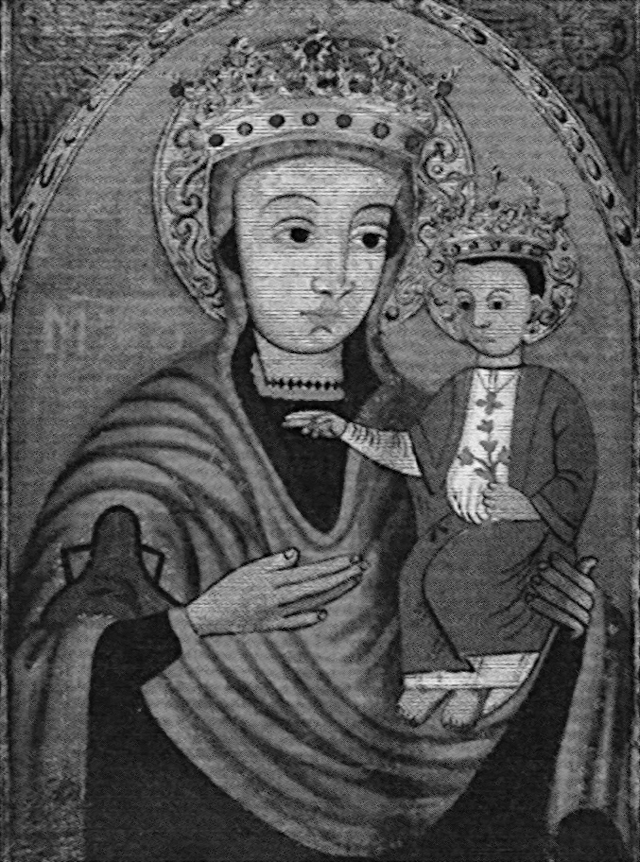
\includegraphics[width=\textwidth]{angolo.png}
\end{minipage}
\hfill
\begin{minipage}{0.72\textwidth}
Confessioni: cogliamo l’occasione per celebrare la festa con il sacramento della Riconciliazione.

Invochiamo con fiducia Maria, la Madre di Gesù e della Chiesa, e ascoltiamo i suoi preziosi consigli, tra i quali insiste nell’accostarci alla confessione e alla Eucarestia nei giorni di festa.
\end{minipage}

\end{center}


\normalsize
